\documentclass[../../syllabus_2.tex]{subfiles}
\begin{document}

\chapter{Les équations}

\faIcon{book} Théorie pages 147 à 151
\section{Introduction}
\subsection{Casse-tête carré (1\iere{} rencontre)}
\begin{center}
  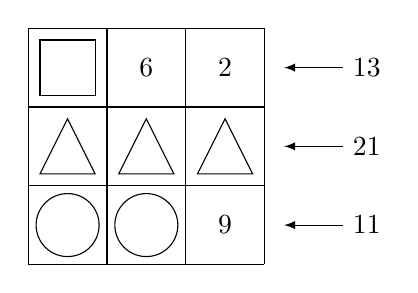
\begin{tikzpicture}
    \draw (0,0) grid (3,3);
    % first row
    \draw (0.15, 2.15) rectangle (0.85, 2.85); 
    \draw (1.5, 2.5) node{$6$};
    \draw (2.5, 2.5) node{$2$};
    % second rows
    \draw (0.15, 1.15) -- (0.85, 1.15) -- (0.5, 1.85) -- cycle;
    \draw (1.15, 1.15) -- (1.85, 1.15) -- (1.5, 1.85) -- cycle;
    \draw (2.15, 1.15) -- (2.85, 1.15) -- (2.5, 1.85) -- cycle;
    % third row
    \draw (0.5, 0.5) circle (0.4 cm);
    \draw (1.5, 0.5) circle (0.4 cm);
    \draw (2.5, 0.5)node{$9$};
    % arrow 
    \draw[<-, >=latex] (3.25, 0.5) -- (4,0.5)node[right]{$11$};
    \draw[<-, >=latex] (3.25, 1.5) -- (4,1.5)node[right]{$21$};
    \draw[<-, >=latex] (3.25, 2.5) -- (4,2.5)node[right]{$13$};
\end{tikzpicture}
\end{center}

Le but de ce casse-tête est de trouver les valeurs cachées sous les
symboles pour que la somme de chaque ligne corresponde au nombre indiqué à côté de celles-ci.

\begin{enumerate}
  \item Observe la première ligne du carré~: si $x$ désigne le symbole $\square$, écris une égalité traduisant la situation. Réduis ensuite les termes
        semblables.\vspace*{2cm}
  \item La première balance à l'équilibre ci-dessous peut représenter cette égalité. Complète le plateau de droite dans la deuxième balance pour
        conserver l'égalité.
        \begin{center}
          \balance{\fbox{$x$}\quad\fbox{8}}{\fbox{13}}
          \hfil
          \balance{\fbox{$x$}}{\fbox{\phantom{11}}}
        \end{center}
  \item
        Quelle manipulation a-t-on effectuée pour conserver l'équilibre de la balance en passant de la première à la seconde~?
        \adf{2}
  \item
        En t'inspirant de cette manipulation, écris la résolution de l'équation.
        \vspace*{3cm}
\end{enumerate}

\begin{exercise}
  Sur base de l'exemple ci-dessus, résous les équations suivantes de type
  $a+x=b$. Laisse ta démarche visible et n'oublie pas d'aligner les égalités.
  \begin{enumerate}[cols=2, itemsep=3cm]
    \item $x + 7 = 13$
    \item $20 = x - 8$
    \item $x - 15 = 0$
    \item $\dfrac{1}{2} + x = 5$
    \item $5 + x = 2$
    \item $3 + x = 20$
    \item $-2 + x = 3$
    \item $ x -\dfrac{3}{4} = -\dfrac{6}{5}$
  \end{enumerate}
  \vspace*{3cm}
\end{exercise}

\newpage
\subsection{Casse-tête carré (2\ieme{} rencontre)}

Reprenons notre casse-tête du début, et intéressons-nous à la deuxième
ligne cette fois.
\begin{center}
  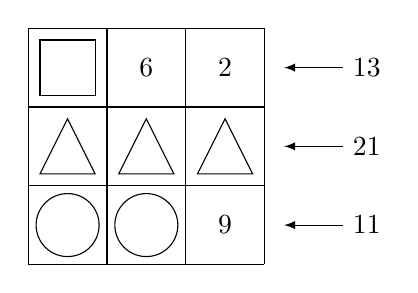
\begin{tikzpicture}
    \draw (0,0) grid (3,3);
    % first row
    \draw (0.15, 2.15) rectangle (0.85, 2.85); 
    \draw (1.5, 2.5) node{$6$};
    \draw (2.5, 2.5) node{$2$};
    % second rows
    \draw (0.15, 1.15) -- (0.85, 1.15) -- (0.5, 1.85) -- cycle;
    \draw (1.15, 1.15) -- (1.85, 1.15) -- (1.5, 1.85) -- cycle;
    \draw (2.15, 1.15) -- (2.85, 1.15) -- (2.5, 1.85) -- cycle;
    % third row
    \draw (0.5, 0.5) circle (0.4 cm);
    \draw (1.5, 0.5) circle (0.4 cm);
    \draw (2.5, 0.5)node{$9$};
    % arrow 
    \draw[<-, >=latex] (3.25, 0.5) -- (4,0.5)node[right]{$11$};
    \draw[<-, >=latex] (3.25, 1.5) -- (4,1.5)node[right]{$21$};
    \draw[<-, >=latex] (3.25, 2.5) -- (4,2.5)node[right]{$13$};
\end{tikzpicture}
\end{center}

\begin{enumerate}
  \item
        Si $x$ désigne le symbole $\triangle$, écris une égalité traduisant la
        situation. Réduis ensuite les termes semblables.\vspace*{2cm}
  \item
        La première balance à l'équilibre ci-dessous peut représenter cette
        égalité. Complète le plateau de droite dans la deuxième balance pour
        conserver l'égalité.
        \begin{center}
          \balance{\fbox{$x$}\quad\fbox{$x$}\quad\fbox{$x$}}{\fbox{21}}
          \hfil
          \balance{\fbox{$x$}}{\fbox{\phantom{11}}}
        \end{center}
  \item
        Quelle manipulation a-t-on effectuée pour conserver l'équilibre de la
        balance en passant de la première à la seconde~?
        \adf{2}
  \item
        En t'inspirant de cette manipulation, écris la résolution de
        l'équation. \vspace*{3cm}
  \item
        Situation similaire~? Complète la deuxième balance pour conserver
        l'équilibre.
        \begin{center}
          \balance{\fbox{$\frac{x}{2}$}}{\fbox{12}}
          \hfil
          \balance{\fbox{$x$}}{\fbox{\phantom{11}}}
        \end{center}
  \item
        Quelle manipulation a-t-on effectuée pour conserver l'équilibre de la
        balance~?
        \adf{2}
  \item
        En t'inspirant de cette manipulation, complète la résolution de
        l'équation.\vspace*{3cm}
\end{enumerate}

\begin{exercise}
  Résous les équations suivantes de type $ax = b$ en laissant visibles
  tes étapes.
  \begin{enumerate}[cols=2, itemsep=3cm]
    \item $7x = 42$
    \item $891 = 3x$
    \item $48 = \dfrac{x}{2}$
    \item $- 6x = 702$
    \item $\dfrac{x}{15} = -25$
    \item $- 3x = 9$
    \item $10x = 0$
    \item $12x = 1$
    \item $-2x=90$
    \item $6x=54$
  \end{enumerate}
  \vspace*{3cm}
\end{exercise}

\newpage
\subsection{Casse-tête carré (3\ieme{} rencontre)}

Il nous reste maintenant la dernière ligne de notre casse-tête à
analyser.
\begin{center}
  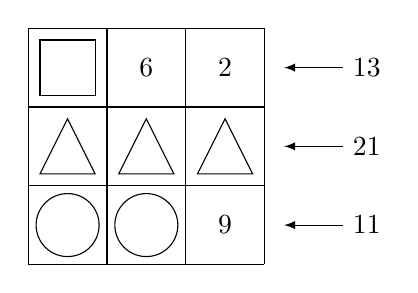
\begin{tikzpicture}
    \draw (0,0) grid (3,3);
    % first row
    \draw (0.15, 2.15) rectangle (0.85, 2.85); 
    \draw (1.5, 2.5) node{$6$};
    \draw (2.5, 2.5) node{$2$};
    % second rows
    \draw (0.15, 1.15) -- (0.85, 1.15) -- (0.5, 1.85) -- cycle;
    \draw (1.15, 1.15) -- (1.85, 1.15) -- (1.5, 1.85) -- cycle;
    \draw (2.15, 1.15) -- (2.85, 1.15) -- (2.5, 1.85) -- cycle;
    % third row
    \draw (0.5, 0.5) circle (0.4 cm);
    \draw (1.5, 0.5) circle (0.4 cm);
    \draw (2.5, 0.5)node{$9$};
    % arrow 
    \draw[<-, >=latex] (3.25, 0.5) -- (4,0.5)node[right]{$11$};
    \draw[<-, >=latex] (3.25, 1.5) -- (4,1.5)node[right]{$21$};
    \draw[<-, >=latex] (3.25, 2.5) -- (4,2.5)node[right]{$13$};
\end{tikzpicture}
\end{center}

\begin{enumerate}
  \item
        Traduis l'égalité suggérée par la dernière ligne en une égalité où
        $x$ représente la valeur du symbole $\bigcirc$ et réduis les termes semblables. \vspace*{2cm}
  \item Pour résoudre cette équation, tu vas devoir combiner les méthodes que tu viens d'apprendre. Peux-tu y arriver ?
        \vspace*{2cm}
\end{enumerate}%

\begin{exercise}
  Résous les équations suivantes de type $ax + b = c$. Laisse ta
  démarche visible.
  \begin{enumerate}[cols=2, itemsep=3cm]
    \item $3x + 7 = 37$
    \item $- 12 = 9x - 3$
    \item $2x + 7 - 6x = - 33$
    \item $6x - 15 = - 2$
    \item $125 = 3x + 17$
    \item $41 = 6x - 1$
  \end{enumerate}
  \vspace*{3cm}
\end{exercise}

\newpage
\section{Vocabulaire}
\adf[Une équation est ]{2}


\vspace*{1cm}\exemple\vspace*{1cm} % espace car il y aura des annotations dans l'exemple

\adf[Résoudre une équation, c'est]{2}

\begin{exercise}
  Associe chaque équation avec sa solution.
  \begin{center}
    $\begin{tblr}{column{2,3}={c,1cm}, rowsep=1ex}
      - 3x = 21       &\bullet  &\bullet &  4   \\
      x + 8 = 12      &\bullet  &\bullet & 7   \\
      2x - 9 = - 17   &\bullet  &\bullet & 5   \\
      10 + 3x = 31    &\bullet  &\bullet & - 7 \\
      17 - x = 3x - 3 &\bullet  &\bullet & - 4 
    \end{tblr}$
  \end{center}
\end{exercise}

\begin{exercise}
  Pour chaque énoncé, détermine si le nombre proposé est solution de
  l'équation.
  \begin{enumerate}[itemsep=4cm]
    \item
          $- 3$ est-il solution de l'équation $5x + 9 = - x + 12$?\newpage
    \item
          $7$ est-il solution de l'équation $5x - 3 = (x - 3) \cdot 8$?
    \item
          $2$ est-il solution de l'équation
          $3x^{2} + 12 = 9x - x^{3} + 14$~?
  \end{enumerate}
  \vspace*{4cm}
\end{exercise}

Voici quelques observations.
\begin{itemize}[label=$\bullet$]
  \item $x +2 = 3 $ est une équation du premier degré à une inconnue.
  \item $x + y = 4$ est une équation du premier degré en $x$ et en $y$ à deux inconnues.
  \item $x^2 = 4 $ est une équation du second degré à une inconnue.
  \item $x^2 + 3 = x$ est une équation du second degré à une inconnue.
\end{itemize}
Peux-tu donner un exemple d'une équation du troisième degré à une inconnue ?
\vspace*{1cm}

\adf[Le degré d'une équation à une inconnue est ]{2}

\faIcon{info-circle} Dans le cadre du cours, nous ne travaillerons qu'avec des équations du premier degré à une inconnue.

\newpage
\section{Méthode de résolution}

Pour résoudre une équation, nous devons isoler l'inconnue (conventionnellement désignée par la lettre $x$) dans un des membres de l'équation. À cette fin, nous avons découvert que nous pouvions effectuer des opérations sur les deux membres de l'égalité sans en changer la solution.

\begin{tcolorbox}[title=Les principes d'équivalences]
  Si on ajoute (retire) un même nombre aux deux membres de l'égalité, alors on obtient une nouvelle égalité qui a la même solution (équivalente).
  \begin{equation*}
    \begin{aligned}
     \tikzmark{a} && x-2 & = 3 &&\tikzmark{c}\\
     \tikzmark{b} && x   & = 5 &&\tikzmark{d} 
   \end{aligned}
\end{equation*}

\begin{tikzpicture}[overlay, remember picture, >=latex]
    \draw[->] ($(pic cs:a)+(0,.5\xlen)$) to[bend right]node[left]{$+2$} ($(pic cs:b)+(0,.5\xlen)$);
    \draw[->] ($(pic cs:c)+(0,.5\xlen)$) to[bend left]node[right]{$+2$} ($(pic cs:d)+(0,.5\xlen)$);
\end{tikzpicture}

  Si on multiplie (divise) par un même nombre non nul les deux membres d'une égalité, alors on obtient une nouvelle égalité qui a la même solution (équivalente).
  \begin{equation*}
    \begin{aligned}
     \tikzmark{e} && 2x & = 10 &&\tikzmark{g}\\
     \tikzmark{f} && x   & = 5 &&\tikzmark{h} 
   \end{aligned}
\end{equation*}

\begin{tikzpicture}[overlay, remember picture, >=latex]
    \draw[->] ($(pic cs:e)+(0,.5\xlen)$) to[bend right]node[left]{$:~2$} ($(pic cs:f)+(0,.5\xlen)$);
    \draw[->] ($(pic cs:g)+(0,.5\xlen)$) to[bend left]node[right]{$:~2$} ($(pic cs:h)+(0,.5\xlen)$);
\end{tikzpicture}
\end{tcolorbox}


Lorsque la résolution d'une équation demande plusieurs étapes, on
respecte l'ordre de la priorité des opérations, mais \og~à l'envers~\fg{}. On
neutralise donc d'abord \emph{les additions et les soustractions}
avant de s'attaquer \emph{aux multiplications et aux divisions}. Plus généralement, on commence par s'occuper de l'opération principale, c'est-à-dire la dernière opération effectuée en suivant la priorité des opérations.

\exemples
\begin{enumerate}[cols=2]
  \item $3x+7=64$
  \item $-12 = -27x+45$
\end{enumerate}
\vspace*{5cm}

\faIcon{info-circle} Le résultat d'une équation peut être une fraction. Veille
  cependant à toujours la simplifier au maximum !

\minisec{Équations avec une inconnue dans les deux membres}

Lorsque nous avons une \emph{inconnue dans chacun des membres}, nous
allons dans un premier temps éliminer les inconnues dans l'un des deux
membres (on dit qu'on isole l'inconnue). Ensuite, nous utiliserons les principes d'équivalences pour déterminer la valeur de cette inconnue.
\begin{align*}
  2x + 5 &= x - 3\\
  \intertext{On peut décide d'isoler $x$ dans le membre de gauche ou de droite. Ici on choisit le membre de gauche en retirant $x$ dans les deux membres}
  x + 5 &= -3\\
  x &= -8
\end{align*}

\exemples
\begin{enumerate}[cols=2]
  \item $3x + 17 = 5x - 25$
  \item $5x+7=9x+17$
\end{enumerate}
\vspace*{5cm}

\begin{exercise}
  Résous les équations suivantes.
  \begin{enumerate}[cols=2]
    \item $16x+9=19x+2$
    \item $13x+9=11x+4$
  \end{enumerate}
  \newpage
  \begin{enumerate}[cols=2, resume]
    \item $2(x + 3) - 9x = 12x + 2$
    \item $10x+5=17x+3$
  \end{enumerate}
  \vspace*{5cm}
\end{exercise}

\minisec{Équations avec des fractions dans les deux membres}
Les principes d'équivalences, nous permettent de facilement transformer une équation contenant des fractions en une équation équivalente qui n'en contient plus. Pour cela, nous allons mettre les deux membres sur le même dénominateur puis les multiplier par ce même dénominateur simplifiant ainsi les fractions.
\begin{align*}
  \dfrac{3}{2} + \dfrac{x}{7} &= \dfrac{15}{14}\\
  \intertext{Mettons toutes ces fractions au même dénominateurs}
  \dfrac{21}{14} + \dfrac{2x}{14} &= \dfrac{15}{14}\\
  \intertext{Multiplions les deux membres par 14 pour simplifier toutes les fractions}
  21 + 2x &= 15\\
  2x &= -6\\
  x &= -3
\end{align*}
\newpage
\begin{exercise}
  Résous les équations suivantes.
  \begin{enumerate}[cols=2, itemsep=6cm]
    \item $\dfrac{5}{8} = \dfrac{9}{x}$
    \item $9 - \dfrac{3}{9} = x - 12x$
    \item $\dfrac{8}{x} = - 16$
    \item $\dfrac{x - 9}{8} + 3 = \dfrac{7}{2}$
    \item $\dfrac{- 3 - x}{4x} = \dfrac{7}{9}$
    \item $\dfrac{14x}{5} = 15$
  \end{enumerate}
  \vspace*{6cm}
\end{exercise}

\newpage
\section{Mise en équation et résolution de problèmes}
Les équations sont un outil très puissant pour trouver des solutions dans des situations concrètes. La difficulté est essentiellement de convertir notre problématique en une équation. Pour t'aider, tu trouveras à la page 151 du manuel de théorie 5 étapes pour résoudre un problème à l'aide d'équations.

\begin{exercise}
  Associe chaque énoncé avec l'équation correspondante.

  $(x+2)\cdot 4 = 50$\hfil
  $50+2=4x$\hfil
  $(x-2)\cdot 4 = 50$\hfil
  $50-20=4x$\hfil
  $2x+50 = 4x$

  \begin{enumerate}
    \item Dimitri pense à un nombre, lui retranche $2$. Puis, il multiplie le résultat par $4$. Il obtient $50$. Quel est ce nombre~? 
    \item Mathilde réserve des places pour se rendre avec trois amies à un concert. Sur son billet de 50~€, on lui rend 20~€. Quel est le prix d'une place~? 
    \item On a augmenté de \SI{2}{cm} chacun des côtés d'un carré. Le périmètre du carré agrandi vaut \SI{50}{cm}. Que mesurait le carré avant l'agrandissement ? 
    \item Un éleveur de chiens a disposé \SI{50}{m} de clôture pour entourer un enclos carré. Il a laissé une ouverture de \SI{2}{m} sans clôture sur un des côtés pour la porte. Quelle est la mesure d'un côté de l'enclos~? 
    \item Théo choisit un nombre, le multiplie par $2$, puis ajoute $50$. Tom multiplie par $4$ le nombre choisi par Théo et obtient le même résultat. Quel était ce nombre~? 
  \end{enumerate}
\end{exercise}

\begin{exercise}
  Si $x$ représente le prix d'une place au tarif \og~ado~\fg{}, entoure l'équation qui correspond au problème posé. Résous ensuite l'équation choisie.

  Un groupe de 8 ados part au théâtre avec 3 adultes. Une place \og~ado~\fg{} est 3~€ moins cher qu'une place \og~adulte~\fg{}. Les 11 personnes ont payé 86~€ au total. Détermine le prix d'une place au tarif \og~ado~\fg{}.
  \begin{enumerate}[cols=2]
    \item $8x+3(x+3)=86$
    \item $8x+3(x-3)=86$
    \item $8x-3(x+3)=86$
    \item $8x-3(x-3)=86$
  \end{enumerate}
  Résolution : \vspace*{5cm}
\end{exercise}

\begin{exercise}
  Résous les problèmes suivants en utilisant les 5 étapes de la page 151 du manuel de théorie.
  \begin{enumerate}[itemsep=10cm]
    \item Jean et sa s\oe{}ur perçoivent leur rétribution pour un travail de
          vacances. La s\oe{}ur de Jean perçoit 100~€ de plus que Jean ;
          ensemble, ils ont \np{1000}~€. Combien ont-ils chacun gagné~?
    \item Victor, Maxence et Zoé ont cueilli $152$ pommes. Maxence en a
          cueilli deux fois plus que Victor et Zoé en a cueilli douze de plus
          que Maxence. Combien de pommes ont-ils chacun cueillies~?
    \newpage
    \item La somme de $3$ nombres consécutifs vaut $129$. Quels sont ces
          nombres~?
    \item Détermine la mesure de $b$ dans la figure suivante si tu sais que son
          périmètre vaut $56$.
          \begin{center}
            \begin{tikzpicture}[scale=0.7, baseline=(current bounding box.north)]
    \draw (0,0) -- (4,0) -- (4,2)node[midway, sloped]{W}node[midway, right=1ex]{$5$} -- (2,2)node[midway,sloped]{W} -- (2,5)node[midway, right=1ex]{$b$} -- (0,5)node[midway, sloped]{W} -- cycle; 
\end{tikzpicture}
          \end{center}
    \newpage
    \item Les $\dfrac{2}{3}$ d'un nombre augmentés ensuite de $10$ valent $60$.
          Quel est ce nombre~?
    \item Le périmètre du petit magasin de bricolage de ta ville (qui est
          représentée par le plan ci-contre) est égal à \SI{62}{m}.
          \begin{center}
            \begin{tikzpicture}
    \tkzDefPoints{0/0/A, 6/0/B, 6/2/C, 4/2/D, 4/3/E, 0/3/F}
    \tkzDrawPolygon(A,B,C,D,E,F)
    \tkzLabelSegment[right](B,C){$x$}
    \tkzLabelSegment[above](C,D){$x$}
    \tkzLabelSegment[right](D,E){\SI{3}{m}}
    \tkzLabelSegment[above](E,F){$2x$}
\end{tikzpicture}
          \end{center}
  \end{enumerate}
\end{exercise}

\newpage
\section{Exercices mélangés}
\subsection{Exercices de drill}
\setcounter{exercise}{0}
\begin{exercise}
  Résous les équations suivantes.
  \begin{enumerate}[cols=3, itemsep=0.4cm]
    \item \(x + 3 = 6\)
    \item \(2=x-4\)
    \item \(-x + 5 = -6\)
    \item \(x - \dfrac{1}{2} = 10\)
    \item \(-8=x + 3\)
    \item \(10=9-(-2x)\)
    \item \(\dfrac{3}{2}+3x=2\)
    \item \(-16=-5x-1\)
    \item \(5x-3=-23\)
    \item \(7=9-2x\)
    \item \(\dfrac{10}{2} x  = -10\)
    \item \(11- x = -6\)
    \item \(\dfrac{9}{4} x+9=8\)
    \item \(-4=x - 1\)
    \item \(\dfrac{3}{4} x=7\)
    \item \(9x=27\)
    \item \(-3x=9\)
    \item \(9=6+3x\)
    \item \(3+4x=19\)
    \item \(5=2x-12\)
    \item \(-\dfrac{1}{4} x = 8\)
    \item \(-x+32=27\)
    \item \(2x+9=21\)
    \item \(12=-5x+ 5\)
  \end{enumerate}
\end{exercise}

\begin{exercise}
  Résous les équations suivantes.
  \begin{enumerate}[cols=2, itemsep=0.4cm]
    \item \(\dfrac{1}{2}+3x=\dfrac{4}{3}\)
    \item \(55x-15=75x+18\)
    \item \(2x+\dfrac{7}{3}=1/4\)
    \item \(4x+3=2x-7\)
    \item \(x-1=3x+9\)
    \item \(2x+8\cdot 5-5=7\cdot 3x\)
    \item \(-14+5x\cdot 2=x+5\)
    \item \(\dfrac{2x}{3}-\dfrac{5x}{4}+5=-6x+\dfrac{4}{3}\)
    \item \(12x+4=88x-16\)
    \item \(-8-8x+2=-6x+x\)
    \item \(19+3x-5x+1=11x\)
    \item \(\dfrac{-5}{2}+\dfrac{2x}{3}+x=\dfrac{4}{3}\)
    \item \(-7x+\dfrac{21}{3}=-43+2x\)
    \item \(\dfrac{6x}{7}+0,2=-x-\dfrac{3}{21}  \)
    \item \( 2x+\dfrac{7}{3}=\dfrac{1}{4}\)
    \item \(9-2x=7x+1\)
    \item \(-125x-25x=80-10x \)
    \item \(\dfrac{-8x}{15}+\dfrac{2}{5}=0,25x+7\)
    \item \(-36+56-2x=18x\)
    \item \(-18+45x+2x=50x\)
    \item \(-14+5x\cdot 2=x+5\)
  \end{enumerate}
\end{exercise}

\newpage
\subsection{À toi de jouer !}
\begin{exercise}
  Vérifie si les valeurs de $x$ sont des solutions des équations
  suivantes.
  \begin{enumerate}
    \item $5$ est-il une solution de l'équation $3x + 7 = 24 - 2$
    \item $17$ est-il solution de l'équation $15 + 2(x - 6) = 32 + x$
    \item $\dfrac{3}{2}$ est-il solution de l'équation
          $6x - 10 = \dfrac{15}{30} - x$
    \item $3$ est-il solution de l'équation
          $x^{2} + 2x - 10 = 2\left( \dfrac{x}{2} + 1 \right)$
  \end{enumerate}
\end{exercise}

\begin{exercise}
  Résous les équations suivantes.
  \begin{enumerate}[cols=2]
    \item $4 + 2x = 20 - 8x$
    \item $2(3x - 1) - 2x = 7x + 3$
    \item $5x + 2 = 2x + 6$
    \item $2x(2x + 3) = - 2x(-x - 7) - (8 - 2x^2)$
    \item $\dfrac{2x - 3}{3} =  - 5x + 1$
    \item $\dfrac{3 - 4x}{5} = \dfrac{2x + 1}{4}$
    \item $(9x - 3)^{2} + 12 = 17 + 81x^2$
    \item $\dfrac{x}{4} = 3$
    \item $3x - 7 + 2x = 8$
    \item $2x - 6 = 5 + x$
    \item $20 = 8x + 2x$
    \item $6x = \dfrac{6}{3}$
    \item $- 3x + 5 = - 1$
    \item $(3 + 2x)^{2} = 5x + 4x^2$
    \item $3(x + 3) = 3x + 9$
    \item $\dfrac{12}{x} + 3 = 6$
    \item $7(5 - 2x)+5 = 45$
    \item $- 7x = \dfrac{5}{6}$
    \item $(x - 9)(1 + x) - 7 = x^2$
    \item $- (5 - x) + 2x = 5x$
  \end{enumerate}
\end{exercise}

\begin{exercise}
  Résous les problèmes suivants. Le résultat peut être un nombre décimal.
  \begin{enumerate}
    \item Squeezie, McFly et Carlito font une vidéo où ils déballent $33$
          objets bizarres. McFly en a déballé $3$ de plus que Carlito et
          Squeezie en a déballé en double de McFly. Combien chacun des
          youtubeurs a-t-il déballé d'objets~?

    \item Les $\dfrac{7}{8}$ d'un nombre valent $6$. Quel est ce nombre~?

    \item Le père de Mirdel a $36$ ans. Si Mirdel était deux fois plus âgé, il
          aurait $10$ ans de moins que son père. Quel est l'âge de Mirdel~?

    \item Pour le projet \og~La VF fait son tour du monde~\fg{}, les élèves de
          2\ieme H ont comptabilisé leurs kilomètres pendant 2
          semaines. Isis annonce~: \og~Margaux a fait \SI{3}{km} de plus que Alexis,
          qui en a fait le tiers seulement de Mehmet. Moi, j'en ai fait autant
          que Mehmet. Au total, à nous quatre, nous avons marché \SI{35}{km}~\fg{}.
          Combien chacun du groupe a-t-il marché de kilomètres~?

    \item Donovan fait un tour de magie. Il dit à Joyca de choisir un nombre, de
          le multiplier par $3$. Ensuite, il lui demande d'ajouter $5$ à son
          produit et de multiplier le tout par $2$. Joyca dit alors qu'il
          est arrivé à $88$ comme résultat. Aide Donovan à trouver le nombre de
          départ de Joyca.
    \item Un  restaurateur a prévu un dessert à base de figues et de mangues. Il se rend chez son grossiste habituel. Les figues se vendent 50 cents pièce et les mangues 1,5 euro chacune. Au total, il a payé 26 € pour 28 fruits. Combien a-t-il acheté de figues ?
    \item Pour  se rendre à une exposition, 4 personnes partent en voiture, 6 vont à pied et le reste remplit 3 minibus.
    Au retour, 9 vont en voiture, 10 vont à pied et le reste remplit 2 minibus.
    Combien de personnes un minibus contient-il ?
    \item Émile  a 15 € et Giulia a 4,5 €. Ils reçoivent alors la même somme d'argent. Après quoi, Émile a trois fois plus d'argent que Giulia. Quel est le montant recu ?
    \item Corentin est maintenant deux fois plus âgé que sa sœur Maëline. Il y a trois ans, ils avaient ensemble 36 ans. Quel est l'âge de Maëline?
    \item Dans un magasin d'ordinateurs, le gérant vend pour 6206 € de matériel informatique : 3 ordinateurs portables, 5 ordinateurs fixes et 4 tablettes. Un ordinateur fixe coûte 170 € de plus qu'un ordinateur portable et le prix d'une tablette vaut 60\% du prix d'un ordinateur portable. Quel est le prix pour un ordinateur portable ?
    \item Les élèves de ton école partent pour une journée « Kayak ». Pour cette activité, l'école paie 612 € pour le bus et 10 € par élève. Au total, l'école a payé 1182 €. Combien d'élèves participent-ils au voyage?
    \item Élise, Laura et Caroline ont ensemble 120 €. Laura possède le double d'Élise et Caroline 8  € de moins qu'Élise. Que possède chacune des filles ?
    \item Détermine la valeur de x pour que le périmètre de ce triangle soit de 109 cm.
    \begin{center}
      
\includegraphics{chapitres/equations/figures/perim.png}
    \end{center}
    \item Un sac contient 35 kg de farine et un autre en contient 25. On verse une partie de la farine du premier sac dans le second. À la fin, le second contient 3 fois plus de farine que le premier. Ouelle est la masse de farine transvasée ?
    \item Il y a une épidémie de grippe dans l'école et un dixième des élèves est absent. Après avoir pris les présences, l'éducateur constate qu'il ne reste plus que 234 élèves ! Avec ces renseignements, détermine le nombre d'élèves dans l'école. 
  \end{enumerate}
\end{exercise}
\end{document}